\documentclass{article}
\usepackage{amssymb}
\usepackage{url}
\usepackage{amsmath}
\usepackage{mathrsfs}
\usepackage{enumerate}
\usepackage{amsthm}
\usepackage{xspace}
\usepackage[utf8]{inputenc}
\usepackage{algorithmicx}
\usepackage{algpseudocode}
\usepackage{tikz}
\usepackage{graphicx}
\usetikzlibrary{shapes,shapes.geometric,arrows,automata}
\usepackage{graphicx}

\newtheorem{lemma}{Lemma}
\newtheorem{theorem}{Theorem}
\newtheorem{corollary}{Corollary}
\newtheorem{example}{Example}
\newtheorem{definition}{Definition}
\newcommand{\nequiv}{{\not\equiv}}
\newcommand{\N}{{\mathbb N}}

\def\Sim{\textit{Sim}}
\def\Merged{\textit{Merged}}
\def\x{{\rm\bf x}}
\def\fpartial{\stackrel{\circ}{\longrightarrow}}
\def\imagetop#1{\vtop{\null\hbox{#1}}}

\newcommand{\card}[1]{|#1|}
\newcommand{\dfa}{DFA\xspace}
\newcommand{\nfa}{NFA\xspace}
\newcommand{\dfas}{DFAs\xspace}
\newcommand{\nfas}{NFAs\xspace}
\newcommand{\comp}[1]{\overline{#1}}
\newcommand{\suff}[1]{\mathsf{suff}(#1)}
\newcommand{\preff}[1]{\mathsf{pref}(#1)}
\newcommand{\inff}[1]{\mathsf{infix}(#1)}
\newcommand{\suffo}{\mathsf{suff}}
\newcommand{\preffo}{\mathsf{pref}}
\newcommand{\inffo}{\mathsf{infix}}
\newcommand{\Succ}[1]{\mathsf{Succ}(#1)}
\newcommand{\disw}[2]{\mathsf{D}_{#1}(#2)}
\newcommand{\dis}[1]{\mathsf{D}(#1)}
\newcommand{\diso}{\mathsf{D}}
\newcommand{\disn}[2]{\mathsf{D}^{#2}(#1)}
\newcommand{\distminw}[2]{\underline{\mathsf{D}}_{#1}(#2)}
\newcommand{\distmin}[1]{\underline{\mathsf{D}}(#1)}
\newcommand{\distmino}{\underline{\mathsf{D}}}
\newcommand{\distminp}[2]{\underline{\mathsf{D}}^{#2}{(#1)}}
\newcommand{\dpre}[1]{\mathsf{E}(#1)}
\newcommand{\dpreo}{\mathsf{E}}
\newcommand{\dpremin}[1]{\underline{\mathsf{E}}(#1)}
\newcommand{\dpreminw}[2]{\underline{\mathsf{E}}_{#1}(#2)}
\newcommand{\dprew}[2]{\mathsf{E}_{#1}(#2)}
\newcommand{\dpren}[2]{\mathsf{E}^{#2}(#1)}
\newcommand{\dpremino}{\underline{\mathsf{E}}}
\newcommand{\dpreminp}[2]{\underline{\mathsf{E}}^{#2}{(#1)}}
\newcommand{\dinf}[1]{\mathsf{F}(#1)}
\newcommand{\dinfo}{\mathsf{F}}
\newcommand{\dinfmin}[1]{\underline{\mathsf{F}}(#1)}
\newcommand{\dinfminw}[2]{\underline{\mathsf{F}}_{#2}(#1)}
\newcommand{\dinfn}[2]{\mathsf{F}^{#2}(#1)}
\newcommand{\dinfw}[2]{\mathsf{F}_{#1}(#2)}
\newcommand{\dinfmino}{\underline{\mathsf{F}}}
\newcommand{\notequiv}{\nLeftrightarrow}
\newcommand{\bcop}[1]{\mathsf{O}(#1)}
\newcommand{\bcopo}{\mathsf{O}}
\newcommand{\bcopn}[2]{\mathsf{O}^{#2}(#1)}
\newcommand{\tmpcomment}[1]{\textbf{\large #1}}


\newcommand{\mneq}[1]{\equiv_{#1}}
\newcommand{\mnleq}[1]{\eqsim_{#1}}
\newcommand{\mntseq}[1]{\approxeq_{#1}}

\newtheorem{comment}{Comment}
\date{}
\newcommand{\Set}[1]{\left\{ #1 \right\}}
\newcommand{\kleene}[1]{#1^\star}
\newcommand{\tuple}[1]{\left\langle #1\right\rangle}
\newcommand{\lang}[1]{{\cal L}(#1)}
\newcommand{\AND}{\;\wedge\:}
\sloppy
\title{Distinguishability Operations  and Closures on Regular Languages}
 \author{Cezar C\^ampeanu \\
Department of Computer Science and Information Technology\\
The University of Prince Edward Island, Canada\\ccampeanu@upei.ca
 \and Nelma Moreira
, Rogério Reis\\
 Centro de Matem\'atica e Faculdade de Ci\^e{}ncias da\\
   Universidade do Porto, Portugal  \\
\{nam,rvr\}@dcc.fc.up.pt}
   
\begin{document}
\maketitle

\begin{abstract}
 Given a regular language , we study the language of words , that  distinguish between pairs of different
left-quotients of . We characterize this distinguishability
operation, show that its iteration has always a fixed point,
and we generalize this result to operations derived from closure operators 
and Boolean operators. 
We give an upper bound for the state complexity of the distinguishability operation, 
and prove its tightness.  
We show that the set of minimal words that can be used to distinguish 
between different left-quotients of a language  has at most  elements,
 where  is the state complexity of , and 
 we also study the properties of its iteration. We generalize the results for the languages of words that distinguish between pairs of different right-quotients and two-sided quotients of a language .
\end{abstract}

\section{Introduction}
\label{sec:intro}
Regular languages and operations over them have been extensively
studied  during the last sixty years, the applications of automata
being continuously extended in different areas. 
As a practical example, we can use automata to model various
electronic circuits. The testing of the circuits can be done by
applying several inputs to various pins of a circuit, and checking the output
produced. 
Because in many cases the circuits emulate automata, it is useful to
develop general tools for testing various properties of automata, such
as testing the relation between the response of the circuit for the
same signal, applied to different gates. 
To answer if an automaton is minimal requires to test if two states
are equivalent or not. 
The easiest way to do this is to use as input different words, and see if
for both states, we reach states with the same finality, thus, in case
of a circuit, for both input gates we will get the same value of the output bit.  
However, checking every possible word is a tedious task, and it would
be useful to limit the testing only to the words that can distinguish
between states. 

Therefore, it is worth studying the languages that distinguish between all
non-equivalent states of a given deterministic finite automaton. 
For an automaton   we denote the distinguishing  
language by  and the language of minimal words
distinguishing between all non-equivalent states by . We can also consider the distinguishability 
languages , and  for a regular language, ,
which will distinguish between all non-equivalent words.

The idea of studying word or state distinguishability is not new. 
In 1958, Ginsburg studied the length of the smallest uniform experiment 
which distinguishes the terminal states of a machine 
\cite{ginsburg58:_lengt_of_small_unifor_exper},
and with Spanier in \cite{Ginsburg1960:InputSemigroup}, he studies whether or not 
an arbitrary semigroup can serve as an input for a 
machine that distinguishes between the elements of the input semigroup.
\ A comparable work was done for terminal
distinguishability by Sempere \cite{JoseSempere}, where terminal
 segments of automata are studied to characterize language 
 families that can be identified in the limit from positive data.  
Indeed, knowing that an automaton  has at most 
states, and having the language , together with the
words of length at most  that are in the language , we
can recover the initial automaton .  
Note that without the language , any learning
procedure will only approximate the language .  
For example, in case we know  to be the set of all the
words of a language  with length at most , we can infer that
 is a cover language for , but we cannot determine which one of
these cover languages is . 
Thus, any learning procedure would only be able to guess  from ,
and the guess would not be accurate, as the number of cover automata
for a finite language can be staggeringly
high~\cite{campeanu13:_cover_languag_and_implem,CezarAndreiCount}. 
\ In ~\cite{restivo12:_graph_theor_approac_to_autom_minim}, 
Restivo and
Vaglica proposed a graph-theoretical approach to test automata
minimality. For  a given automaton  they associate 
a digraph, called \emph{pair graph}, where vertices are pairs
 of states of , and  edges connect vertices for which
the states have a transition from the same symbol in . Then, two states
 and  of  are distinguishable if and only if there is a path
from the vertex  to a vertex , where  is
final and   is non final, i.e., there exists a word that distinguishes
between them. 
A related research topic is the problem of finding a minimal \dfa that
 distinguishes between two words by accepting one and rejecting the other.
It was studied by~Blumer et
al. in \cite{blumer85:_small_autom_recog_subwor_of_text}, and recently 
Demaine et al. in \cite{demaine11:_remar_separ_words} 
reviewed several attempts to solve the problem and presented new results. 

In the present paper we do not separate two words by a language,
instead, we distinguish between non-equivalent quotients of the same
language. We use many powerful tools such as 
language quotients, atoms, and universal witnesses, 
that hide proof complexity,
helping us to produce a presentation easier to follow.
We introduce the notation in Section~\ref{snotation},  define and
prove general properties of the distinguishability operation in
Section~\ref{sgenres}, and prove some state complexity results in
Section~\ref{ssc}.  
In Section~\ref{sec:minDist}, we analyze the set of minimal words with
respect to quasi-lexicographical order that distinguishes different
quotients of a regular language. 
In Section~\ref{sec:recoverL}, we present an algorithm that can be used
as a positive learning procedure for language  if  is known.
In Section~\ref{sec:sufclosuregeneral}, we present a class of operands using closure operations and Boolean operations, that have a 
fixed point under iteration. 
In Section~\ref{sec:otherdis} we define other distinguishability operations and study their properties.  
The conclusion, together with open problems and future work, are included 
in Section~\ref{sconc}. 


\section{Notation and Definitions}
\label{snotation}
For a set , its cardinality is denoted by . 
An \emph{alphabet}  is a finite non-empty set, and the free monoid
generated by  is . 
A word  is an element of  and a \emph{language} is a subset of .  
The \emph{complement} of a language  is .
The \emph{length} of a word , ,
, , with  is .  
The \emph{empty word} is , and . If  for some  then  is a \emph{prefix} of ,  is a \emph{factor} (or \emph{infix}) of  and  a \emph{suffix} of .
Consider an order over . 
In , we define the \emph{quasi-lexicographical} order as: 
if  or  and  lexicographically precedes . 
The reverse  of a
word  is defined as follows: , and , for . 
The \emph{reverse} of a language  is denoted by  and defined as .

A \emph{deterministic finite automaton} (\dfa) is a quintuple
, where  is  a finite
non-empty set, the set of states,  is the  alphabet,  is the initial state,  is the set of final states,
and  is the transition
function. This function defines for each symbol of
the alphabet a transformation of the set  of states (i.e. a map from  to ). The
\emph{transition semigroup} of a \dfa , 
\cite{bell14:_symmet_group_and_quotien_compl},
 is the semigroup of transformations of  generated 
by the transformations induced by the symbols of .

A \emph{reduced} \dfa is a \dfa with all states reachable from the  
initial state (accessible), and all states can reach a final state 
(useful), except at most one that is a \emph{sink} state or
\emph{dead} state, i.e., a state where all output transitions are self
loops. 


The transition function  can be extended to  by , and
. 
The language recognized by a \dfa  is
.  
We denote by 
 and  the \emph{left} and \emph{right} languages of , respectively,
i.e.,  
, and 
. 

The minimal word in quasi-lexicographical order that reaches state 
is ; the word  is also the minimal element of .

A \emph{regular language} is a language recognized by a \dfa.  
A regular language  
induces on  the Myhill-Nerode equivalence relation:
  if, for all , we have that  if and only if . 
If  is a \dfa recognizing
the language  and  , then we say that  and  are equivalent, 
and write .   
A \dfa is \emph{minimal} if it has no equivalent states.
The \emph{left quotient}, or simply \emph{quotient}, of a regular
language  by a word  is the language . A quotient 
corresponds to an equivalence class of , i.e. two words are equivalent if and only if their quotients are the same. 
If a language  is regular, the number of distinct left quotients is
finite, and it is exactly the number of states in the \emph{minimal} \dfa
recognizing . This number is called the \emph{state complexity} of ,
 and is denoted by . 
In a minimal \dfa, for each ,  is exactly a quotient. 
If some quotient of a language  is , this means that the
minimal \dfa of  has a dead state. 

A \emph{nondeterministic finite automata}  (\nfa) is a quintuple
, where , , and
 are the same as in the \dfa definition,  is the set of
initial states, and  is the
transition function.  
The transition function can also be extended to subsets of  instead
of states, and to words instead of symbols of . 
The language recognized by  an \nfa  is
.  
It is obvious that a \dfa is also an \nfa. 
Any \nfa can be converted in an equivalent \dfa by the well known
\emph{subset construction}. Given an \nfa  for , an \nfa  for  is obtained by interchanging the sets of final and initial states of  and reversing all transitions between states.

More notation and definitions related to formal languages can be consulted in~\cite{sakarovitch09:_elemen_of_autom_theor,yu97:_handb_formal_languag}.



\section{The (Left) Distinguishability Operation}
\label{sgenres}
Let  be a regular language. 
For every pair of words, , with ,
there exists at least one word  such that either 
or . 
Let   be a \dfa such that
.  
If two states , , then there exists at least one
word  such that .  
We say that  distinguishes between the words  and , in the
first case, and the states  and , in the second case. Given , the language that \emph{distinguishes}  from
 w.r.t.  is 


Naturally, we define the 
\emph{left distinguishability language} (or simply, distinguishability language) of  by


It is immediate that .
In the same way, for the \dfa , we define 
for , and 


\begin{lemma}
 Let  be two reduced \dfas such that 
. 
Then .
\end{lemma}
\begin{proof}
Let  and
.  
It is enough to prove that .
If , then we have two words  such that
 and . 
Let  and . 
Then,  and , so . 
If  , then there exist  such that 
 and  ; as  is reduced, 
there must exist  with  and , 
therefore  and ,
 hence,  and , i.e., we conclude .
\end{proof}

This shows that the operator  is independent of the automata
we choose to represent the language. In what follows, we present some characterization results for the
distinguishability operation, and show that iterating the operation
always leads to a fixed point. 

The distinguishability operation can be expressed directly by means of
the language quotients, as it can be seen in the following result. 
\begin{theorem}
\label{theo:dist-quot}
Let  be a regular language with  its set of (left) quotients. Then we have the equality

\end{theorem}
\begin{proof}
Let , i.e.,
 . 
Then , therefore  
. 

Let , then let  and
 be such that  and . Thus, . Hence, we conclude
 
\end{proof}
\begin{corollary}
\label{cor;diffxyquot}
For a regular language  and ,  is 
the symmetric difference of the correspondent quotients, 

\end{corollary}

To help the reader better understand  how these languages look like, next we present 
some examples.

\begin{example}
\label{ex:singleton}
 If the language  has only one quotient, i.e.,  or
 , then , as there are no
 different quotients to distinguish. 
\end{example}

\begin{example}
\label{ex:epsilon}
If , then we can only distinguish between final 
and non-final states, thus the minimal \dfa of  has exactly two states 
corresponding to its  two quotients.
\end{example}

\begin{example}
\label{ex:symmerysg}
In this example we consider a family of languages  for which .
Let  for ,  with
,  
where , 
, for  and 
, ,  , for .  
In Figure~\ref{fSigmaS}, we present~.   
Both symbols of the alphabet induce permutations on :  induces
a transposition (2-cycle), and  , an  cyclic permutation. It
follows that, the transition semigroup of   
is the symmetric group  of degree , i.e., the set of all
permutations of .  
We always have  , and  
 every  induces a permutation on the states, 
for  ,  and  ,
with .  
Then, there must exist at least a pair , such that  and
, i.e., 
 ,  thus . 
Bell et al.~\cite{bell14:_symmet_group_and_quotien_compl}
studied those families of automata,  
and in particular, proved that they are uniformly minimal, i.e.,
minimal for every non-trivial choice of final
states~\cite{restivo12:_graph_theor_approac_to_autom_minim}.  
\end{example}

\begin{figure}[htb]
\begin{center}

\hfill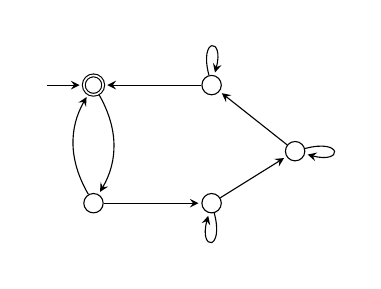
\begin{tikzpicture}[>=stealth, shorten >=1pt, auto, node distance=1.5cm,initial text={}]

\node[state, accepting, initial, inner sep=1pt, minimum size=7pt] (S0){};
\node[state, inner sep=1pt, minimum size=15pt][below of=S0, minimum size=7pt] (S1){};
\node[state, inner sep=1pt, minimum size=15pt][right of=S1,minimum size=7pt] (S2){};
\node[state, inner sep=1pt, minimum size=15pt][above right of=S2, yshift = -.4cm, minimum size=7pt] (S3){};
\node[state, inner sep=1pt, minimum size=15pt][right of=S0, minimum size=7pt] (S4){};
\path[->](S0) edge [bend left]node {} (S1)
         (S1) edge node [swap]{} (S2)
		      edge [bend left] node {} (S0)
		 (S2) edge node [swap]{} (S3)
		      edge [loop below] node {} ()
		 (S3) edge node {} (S4)
		      edge [loop right] node {} ()
		 (S4) edge [loop above] node {} ()
		      edge node [swap] {} (S0);
\end{tikzpicture} \quad
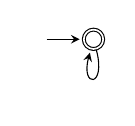
\begin{tikzpicture}[>=stealth, shorten >=1pt, auto, node distance=2cm,initial text={}]

\node[state, accepting, initial, inner sep=1pt, minimum size=7pt] (S0){};
\path[->]
		 (S0) edge [loop below] node {} ();
\end{tikzpicture} \hfill~
\caption{Automaton   (left) and its distinguishability language,   (right).
  } 
\label{fSigmaS} 
\end{center}
\end{figure}
\begin{figure}[h!]
\begin{center}
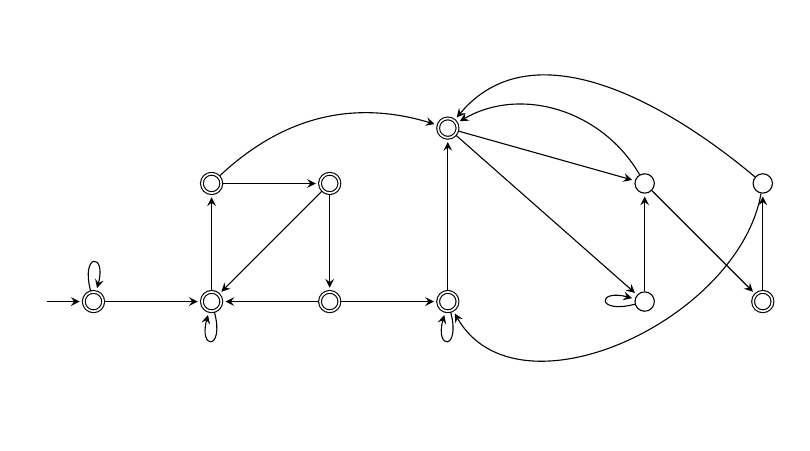
\begin{tikzpicture}[>=stealth, shorten >=1pt, auto, node distance=1.5cm,initial text={}]

\node[state, accepting, initial, inner sep=1pt, minimum size=7pt] (S0){};
\node[state, accepting, inner sep=1pt, minimum size=7pt] [right of=S0](S1){};
\node[state, accepting, inner sep=1pt, minimum size=7pt] [above of=S1](S2){};
\node[state, accepting, inner sep=1pt, minimum size=7pt] [right of=S2](S3){};
\node[state, accepting, inner sep=1pt, minimum size=7pt] [below of=S3](S4){};
\node[state, accepting, inner sep=1pt, minimum size=7pt] [right of=S4](S5){};
\node[state, accepting, inner sep=1pt, minimum size=7pt] [above of=S5, yshift=20pt](S6){};
\node[state, inner sep=1pt, xshift=1cm, minimum size=7pt] [right of=S5](S7){};
\node[state, inner sep=1pt, minimum size=7pt] [above of=S7](S8){};
\node[state, accepting, inner sep=1pt, minimum size=7pt] [right of=S7](S9){};
\node[state, inner sep=1pt, minimum size=7pt] [above of=S9](S10){};
\path[->] (S0) edge [loop above] node {}()
               edge node {}(S1)
		  (S1) edge [loop below] node {}()
		       edge node {}(S2)
		  (S2) edge node {}(S3)
		       edge [bend left] node [pos=.2] {}(S6)
		  (S3) edge node {}(S1)
			   edge node {}(S4)
		  (S4) edge node {}(S1)
		       edge node {}(S5)
		  (S5) edge [loop below] node {}()
		       edge node {}(S6)
		  (S6) edge node {}(S7)
		       edge node [pos=.2]{}(S8)
		  (S7) edge [loop left] node {}()
		       edge node {}(S8)
		  (S8) edge [out=120, in=30] node[swap, pos=.2] {}(S6)
		       edge node [pos=.2]{}(S9)
		  (S9) edge node [swap]{}(S10)
		  (S10) edge [out=140,in=50] node [pos=.1,swap] {}(S6)
		        edge [out=260,in=300] node {} (S5);
\end{tikzpicture} \end{center}
\caption{Example of an automaton with .} 
\label{fdiff} 
\end{figure}

\begin{example}
\label{ex:ts45}
Consider the automaton  in Figure~\ref{fdiff}.\ 
We have that ,  
but .  
The minimal automaton for  is presented in Figure~\ref{ffixp}.
\end{example}

\begin{figure}
\begin{center}
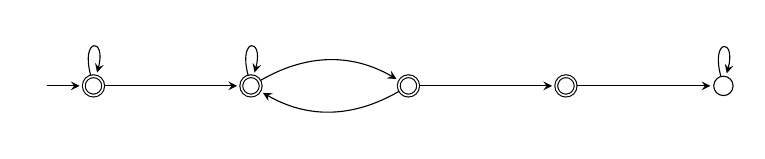
\begin{tikzpicture}[>=stealth, shorten >=1pt, auto, node distance=2cm,initial text={}]

\node[state, accepting, initial, inner sep=1pt, minimum size=7pt] (S0){};
\node[state, accepting, inner sep=1pt, minimum size=7pt] [right of=S0](S1){};
\node[state, accepting, inner sep=1pt, minimum size=7pt] [right of=S1](S2){};
\node[state, accepting, inner sep=1pt, minimum size=7pt] [right of=S2](S3){};
\node[state, inner sep=1pt, minimum size=7pt] [right of=S3](S4){};
\path[->] (S0) edge node {} (S1)
	           edge [loop above] node {}()
		  (S1) edge [loop above] node {}()
		       edge [bend left] node {}(S2)
		  (S2) edge [bend left] node{}(S1)
		       edge node {} (S3)
		  (S3) edge node {} (S4)
		  (S4) edge [loop above] node {}();
\end{tikzpicture} \end{center}
\caption{Example of automaton where , i.e. distinguishability  
language is the same as the language of the words it can distinguish.}
\label{ffixp} 
\end{figure} 


\begin{example}
\label{ex:suff}
Considering the language , 
in Figure~\ref{f1} one can find, from left to right, a \dfa that accepts , 
one that accepts  , 
and one  for  , for .
\end{example}

From the last example, we can see that the language  contains
the word ,  
but also the words , ,  and , which are all suffixes of  . 
This observation suggests that  is suffix closed, which is proved 
in the following theorem.

\begin{figure}[h!]
\hfill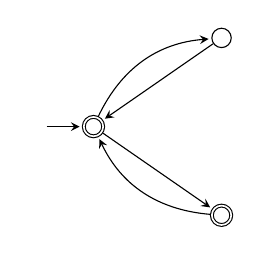
\begin{tikzpicture}[>=stealth, shorten >=1pt, auto, node distance=2.3cm,initial text={}]
\node[state, accepting, initial, inner sep=1pt, minimum size=7pt] (S0){};
\node[state, inner sep=1pt, minimum size=15pt, minimum size=7pt, yshift=-.5cm][above right of=S0] (S1){};
\node[state, accepting, inner sep=1pt, minimum size=15pt, minimum size=7pt, yshift=.5cm][below right of=S0] (S2){};
\path[->](S0) edge [bend left] node{}(S1)
              edge node{}(S2)
		 (S1) edge node{}(S0)
         (S2) edge [bend left] node{}(S0);
\end{tikzpicture} \hfill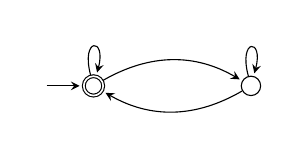
\begin{tikzpicture}[>=stealth, shorten >=1pt, auto, node distance=2cm,initial text={}]
\node[state, accepting, initial, inner sep=1pt, minimum size=7pt] (S0){};
\node[state, inner sep=1pt, minimum size=15pt, minimum size=7pt][right of=S0] (S1){};
\path[->](S0) edge [bend left] node{}(S1)
              edge [loop above] node{}()
		 (S1) edge [bend left] node{}(S0)
		      edge [loop above] node{}();
\end{tikzpicture} \hfill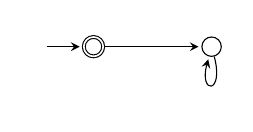
\begin{tikzpicture}[>=stealth, shorten >=1pt, auto, node distance=1.5cm,initial text={}]
\node[state, accepting, initial, inner sep=1pt, minimum size=7pt] (S0){};
\node[state, inner sep=1pt, minimum size=15pt, minimum size=7pt][right of=S0] (S1){};
\path[->] (S0) edge node {} (S1)
          (S1) edge [loop below] node {}();
\end{tikzpicture} \hfill~
\caption{Automata for the languages , , and ,
  .} 
\label{f1}
\end{figure}

\begin{theorem}
\label{tsuffcl}
    If  is a regular language, then the language  is suffix
    closed, i.e.,  
     
\end{theorem}
\begin{proof}
Let , i.e., there exist  such that  
 and . 
If  is a suffix of , i.e., , for an , 
then we can write  and , which means that .
\end{proof}

Using Theorem~\ref{theo:dist-quot}, 
if , then 
 is a suffix of a word in , and a suffix of the complement of ,
because 
 

 Accordingly,
, where  is
the language of all suffixes of . 
If , then we can find  and  such that
 and , thus .
Therefore, we just found a new way to express the distinguishability
language of : 

\begin{theorem}
\label{theo:dss} If  is a regular language, then

\end{theorem}

Because  is suffix closed,  , hence
 and
. 
In general, we have for every , the following inclusion


Consequently, we may ask if this hierarchy is infinite or not, in other words, 
we may ask if for any language ,
there exists  such that . 

\begin{example}
\label{ex:d3}
Consider the language , where  is given 
in Figure~\ref{f2}, on the left. For the language , we have that  and 
 , for . 
The minimal automaton for   is depicted on the right. 
The minimal automaton for  has  states.
\end{example}

\begin{figure}[h!]
\begin{center}
\hfill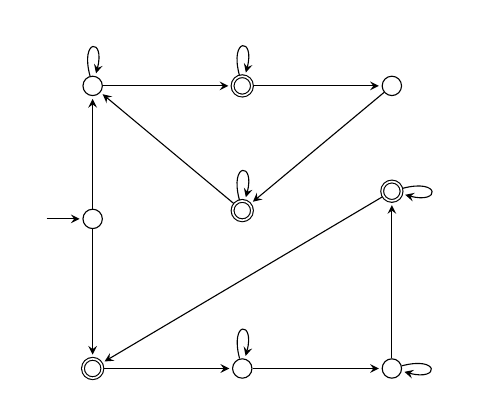
\begin{tikzpicture}[>=stealth, shorten >=1pt, auto, node distance=1.9cm,initial text={}]

\node[state, initial, inner sep=1pt, minimum size=7pt] (S0){};
\node[state, inner sep=1pt, minimum size=7pt][above of=S0,yshift=-6pt] (S1){};
\node[state, accepting, inner sep=1pt, minimum size=7pt][right of=S1] (S2){};
\node[state, inner sep=1pt, minimum size=7pt][right of=S2] (S3){};
\node[state, accepting, inner sep=1pt, minimum size=7pt,yshift=9pt][below of=S2] (S4){};
\node[state, accepting, inner sep=1pt, minimum size=7pt][below of=S0, yshift=-0pt] (S5){};
\node[state, inner sep=1pt, minimum size=7pt][right of=S5] (S6){};
\node[state, inner sep=1pt, minimum size=7pt][right of=S6] (S7){};
\node[state, accepting, inner sep=1pt, minimum size=7pt, yshift=10pt][above of=S7] (S8){};
\path[->] (S0) edge node {}(S1)
               edge node {}(S5)
		  (S1) edge [loop above] node {}()
		       edge node {}(S2)
		  (S2) edge [loop above] node {}()
		       edge node {}(S3)
		  (S3) edge node [pos=.2] {}(S4)
		  (S4) edge [loop above] node {}()
		       edge node {}(S1)
		  (S5) edge node {}(S6)
		  (S6) edge [loop above] node {}()
		       edge node {}(S7)
		  (S7) edge [loop right] node {}()
		       edge node {}(S8)
		  (S8) edge [loop right] node {}()
		       edge node[pos=.3,swap] {}(S5);
\end{tikzpicture} \hfill
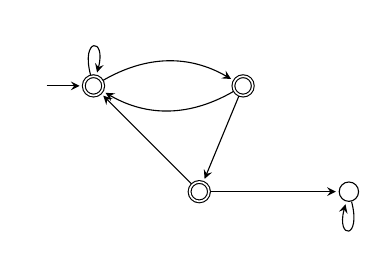
\begin{tikzpicture}[>=stealth, shorten >=1pt, auto, node distance=1.9cm,initial text={}]

\node[state, initial, accepting, inner sep=1pt, minimum size=7pt] (S0){};
\node[state, accepting,inner sep=1pt, minimum size=7pt][right of=S0] (S1){};
\node[state, accepting,inner sep=1pt, minimum size=7pt][below right of=S0] (S2){};
\node[state, inner sep=1pt, minimum size=7pt][right of=S2] (S3){};
\path[->] (S0) edge [loop above] node {}()
			   edge [bend left] node {}(S1)
		  (S1) edge [bend left] node {}(S0)
		       edge node {}(S2)
		  (S2) edge node {}(S0)
		       edge node {}(S3)
		  (S3) edge [loop below] node {}();

\end{tikzpicture} \hfill~
\end{center}
\caption{Example of a language  with
, for . On the left a \dfa for  and on the right a \dfa for .} 
\label{f2}
\end{figure}

The following lemma will be useful for the rest of the section.

\begin{lemma}
\label{lsufcap}
 If  are suffix-closed languages, then
, and 
.
\end{lemma}
\begin{proof}
It is obvious that the equality holds for reunion, and  
the inclusion , for intersection is true.
If , then
there exist  such that  and . 
Because  and  are suffix closed, then

\end{proof}

In the following result, we prove that the iteration of 
operations always reaches a fixed point. 

\begin{theorem}
\label{theo:fixpoint}
Let  be a regular language. 
Then we have that  
  .
\end{theorem}

\begin{proof}
We have the following equalities:

  
Now, computing the next iteration of , we get
 .

Using~(\ref{eq:d2}) and Lemma~\ref{lsufcap},  we obtain the equalities

Because  is a suffix-closed language, it follows that

\end{proof}

The following results give some characterization for the languages
that are fixed points for . 

\begin{lemma}
\label{lem:qempty}
Given a regular language , if  has  as a quotient then .
\end{lemma}

\begin{proof}
Because , for some word , we have that
. 
\end{proof}
This lemma makes the following result immediate.
\begin{theorem}
\label{theo:ldirectdead}
 If  is a suffix closed regular language with  as one of the
 quotients,  then  is a fixed point for , i.e., .
\end{theorem}

\begin{corollary}
\label{cor:emptyquotient}
Let  be a regular language. If  has  as a quotient, then .
 \end{corollary}

Note that suffix-closeness of  is not sufficient to ensure that  has  as quotient.
 For that, it is enough to consider the language given by .
 However, if  is a  fixed point, the implication yields.

\begin{theorem}
\label{ldead}
    Let  be a regular language.
If , then  has  as a quotient. 
\end{theorem}
\begin{proof}
Let  be a regular language that is fixed point for , thus  is suffix closed and 

Assume that  does not have  as quotient, i.e., 

Let  ( is not a fixed point for ). 
Thus by~\eqref{ecological} there  exists a  such that 
 and because  is suffix closed, it follows that . 
Using \eqref{fix-point} there exists  such that . 
Using the same reasoning, we can find  and  such that 

The word  distinguishes  from , thus these words cannot belong to the same quotient. Suppose that we have iterated  times this process having 

with all  belonging to 
distinct quotients. We can apply this process one more time, obtaining 
 
It is easy to see that the word  distinguishes  from 
any of the previous words  (with ) because  is a suffix of .
Thus, the number of  quotients cannot be finite, a contradiction.
\end{proof}

By contraposition over the last result, we get that  a language 
with all its quotients non-empty cannot be a fixed point for . 
 We know that, if a language  is such
that , then  must be one of
the quotients of . 
In Examples~\ref{ex:symmerysg}--\ref{ex:suff}
and Example~\ref{ex:d3}, we have  languages  with all quotients non-empty and  . Considering Theorem~\ref{ldead} and Theorem~\ref{fix-point}, given any regular language  we can iterate  at most two times to obtain a language that has  as a quotient.

For a finite language , 
it follows from Lemma~\ref{lem:qempty}
that the
distinguishability language of  coincides with the set of all suffixes of ,
therefore,  is a fixed point of the  operator.

\begin{corollary}
\label{cor:finite}
  If  is a finite language, then .
\end{corollary}



The minimal \dfa that represents the set of suffixes of a finite
language  is called the \emph{suffix automaton}, and several
optimized algorithms for its construction were studied in the
literature. Thus, we can use an algorithm for building the suffix
automaton  in order to obtain . Recently, Mohri et
al.~\cite{mohri09:_gener_suffix_autom_const_algor} gave new upper
bounds on the number of states of the suffix automaton as a function
of the size of the minimal \dfa of , as well as other measures of
. In Section~\ref{ssc}, we study the state complexity of
 as a function of the state complexity of , for any general regular language . In Section~\ref{sec:sufclosuregeneral}, we generalize the results on the
characterization of the distinguishability operation, defining more operations on regular languages. 

\section{State Complexity}
\label{ssc}
By Theorem~\ref{theo:dss}, we know that  can be obtained  
using the suffix operator, complement and intersection,
therefore, it is a result of combining three operations, two unary and one binary.
We would like to estimate the state complexity of the  operation and 
check if the upper bound is tight.
We recall that the state complexity of an operation is the worst-case state complexity of a language resulting from that operation, as a function of the state complexities of the operands.
 
The following theorem shows the construction for , in case  is recognized by a \dfa.
 
\begin{theorem}
\label{theo:algodis}
  Let  be a  reduced \dfa recognizing a language .\ Then  is a \dfa that accepts , 
where 
\begin{itemize}
 \item , 
 \item for  and  and , 
,
 \item .
\end{itemize}
\end{theorem}
\begin{proof}
Considering that , we can use
the usual subset construction for  to build an \nfa
with the same transition function as , 
and all its states being initial. 
For , the corresponding \nfa will be the same, 
but flipping the finality to all the states.  
Because both operands share the same structure,
the \dfa corresponding to the intersection
 will be the \dfa resulting from the subset construction 
 considering a suitable set of final states
(they must contain at least one final state and a non-final one). 
As all states  with  are either final or non-final, 
they cannot be useful, therefore they can be ignored.
\end{proof}

Let  be the minimal \dfa recognizing
 with . 
Let  and , , be the
left-quotients of  (possibly including the empty set). 
From  Theorem~\ref{theo:dist-quot}, we have:
  

In the following we identify the states of  with the
corresponding left-quotients. 
Instead of using traditional techniques to prove the correctness of 
tight upper bounds of operational state complexity, 
here we consider a method based on the \emph{atoms} 
of regular expressions. 
Using this approach, we  aim to provide yet another piece of evidence for their
 broad applicability.

Brzozowski and Tamm introduced
the notion of atoms of regular languages in~\cite{brzozowski11:_theor_of_atomat}
  and studied their state complexity in~\cite{brzozowski13:_compl_of_atoms_of_regul_languag}. 
An \emph{atom} of a regular language  with  quotients , \ldots,
 is a non-empty intersection ,
where each  is a quotient , or its complement
. Atoms of  are partition of  .
In particular,  
() is an atom with zero complemented 
(uncomplemented) quotients.
In~\cite{brzozowski13:_compl_of_atoms_of_regul_languag} it
was proved that the state complexity of both those atoms is . 
Using similar arguments, we prove the following theorem.

\begin{theorem}
  \label{theo:scdistub}
If a regular language  has a  minimal \dfa with  states, then
. 
\end{theorem}
\begin{proof}
  Let  be the minimal \dfa recognizing
   with . 
Then , and let ,  be the
  (left-)quotients of . 
\ Using Equation~(\ref{eq:atoms}), every quotient 
  of , for , is given by:

\noindent where all , , are also
quotients of , and they may not be distinct. 
Considering all non-empty subsets of quotients of , 
there would be at most  quotients of . 
However, all subsets, , with exactly one element 
will lead to the empty quotient.  Thus, . 
\end{proof}

Brzozowski~\cite{brzozowski13:_in_searc_of_most_compl_regul_languag}
presented a family of languages  which provides witnesses for the
state complexity of several individual and combined operations over
regular languages. Brzozowski and
Tamm~\cite{brzozowski13:_compl_of_atoms_of_regul_languag} proved that
 was also a witness for the worst-case state complexity of
atoms. This family is defined as follows. For each , 
we construct the \dfas , where  
, , ,
 for  
,  for , and . 
We denote by 
the language accepted by , i.e.,

We show that  is also a witness for the lower-bound of the state
complexity of . 
First, observe that automata ,  are minimal. 
In Figure~\ref{fig:univ}, we present .

\begin{figure}[h!]
\begin{center}
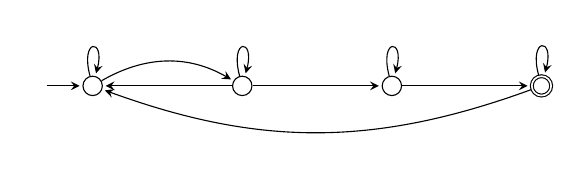
\begin{tikzpicture}[>=stealth, shorten >=1pt, auto, node distance=1.9cm,initial text={}]

\node[state, initial, inner sep=1pt, minimum size=7pt] (S0) {};
\node[state, inner sep=1pt, minimum size=7pt][right of=S0] (S1) {};
\node[state, inner sep=1pt, minimum size=7pt][right of=S1] (S2) {};
\node[state, accepting, inner sep=1pt, minimum size=7pt][right of=S2] (S3) {};
\path[->] (S0) edge [loop above] node {} ()
               edge [bend left] node {} (S1)
		  (S1) edge node {} (S2)
		       edge node [pos=.2]{} (S0)
			   edge [loop above] node {} ()
		  (S2) edge node {} (S3)
		       edge [loop above] node {} ()
		  (S3) edge [loop above] node {} ()
		       edge [in=340, out=200] node [pos=.2]{} (S0);
\end{tikzpicture} \end{center}
\caption{Universal witness .} 
\label{fig:univ} 
\end{figure}
Next, we give the lower bound for the number of states of a 
\dfa accepting .
\begin{theorem}
    \label{theo:scdisttight}
For , the minimal \dfa accepting  has  states.
\end{theorem}
\begin{proof}
  Let , and 
, 
be the two atoms of  as above, where  are its quotients . 
Then .  
Brzozowski and Tamm proved that
  . 
Applying the construction given
  in Theorem~\ref{theo:algodis} to , and noting that a regular language
  and its complement have the same state complexity, we obtain the upper
  bound.
\end{proof}

If , by Example~\ref{ex:singleton}, we have that . If  has  as a quotient, by Lemma~\ref{lem:qempty},  the upper bound for  coincides with the one for , i.e. it is  if ,~\cite{brzozowski14:_quotien_compl_of_closed_languag}. This upper bound is achieved by the family of languages represented in Figure~\ref{fig:upsuffe}.

\begin{figure}[h!]
\begin{center}
\begin{tikzpicture}[>=stealth, shorten >=1pt, auto, node distance=1.9cm,initial text={}]

\node[state, accepting, initial, inner sep=1pt, minimum size=5pt] (S0) {};
\node[state, inner sep=1pt, minimum size=5pt][right of=S0] (S1) {};
\node[state, inner sep=1pt, minimum size=5pt][right of=S1] (S2) {};
\node[right of=S2] (SS) {};
\node[state, inner sep=1pt, minimum size=5pt][right of=SS] (SN2) {};
\node[state, inner sep=1pt, minimum size=5pt][above of=S0] (SN1) {};

\path[->] (S0) edge node {} (S1)
               edge node {} (SN1)
		  (S1) edge node {} (S2)
		       edge [in=345,out=195] node [pos=.2] {} (S0)
		  (S2) edge node {} (SS)
		       edge [loop above] node {} ()
		  (SS) edge node {} (SN2)
		  (SN2) edge [in=335, out = 205] node [pos=.15] {} (S0) 
		       edge [loop above] node {} ()
		  (SN1) edge [loop right] node {} ();
\end{tikzpicture} \end{center}
\caption{Witness family for   when  has  as a quotient.} 
\label{fig:upsuffe} 
\end{figure}
Having considered some  properties of the distinguishability language,
we would like  to select only the set of minimal words that
distinguishes between distinct quotients. Obviously, 
this is a subset of , and in the following  section we study its properties.

\section{Minimal Distinguishable Words}
\label{sec:minDist}
An even more succinct language distinguishing all different quotients
of a regular language, in fact a finite one, can be obtained if we
consider only the shortest word that distinguishes each pair of
quotients.  

\begin{definition}
\label{def:distmin}  
    Let  be a regular language, and assume we have an order over 
the alphabet .
If  and , 
 we define 

where minimum is considered with respect to the quasi-lexicographical order.
In case   ,  is undefined.
We can observe that if , 
.


 The set of minimal words distinguishing quotients of a language  
is 

\end{definition}
 
\begin{example}
\label{ex:dismt} We present a few simple cases. Similar to the  operator, 
we have the equalities:
 and . 
In case , , and 
 , for .
\end{example}

\begin{example}
  \label{ex:dmin}
  Consider the language  of Example~\ref{ex:d3}. 
We have the following equalities
, 
, and  
.
\end{example}

The previous example suggests that  is also suffix closed.
   
\begin{theorem}
\label{theo:mindist_is_suffix_closed}
If  is a regular language, then  is suffix closed.
\end{theorem}
\begin{proof}
  Let , and let , with . 
Because ,
  we can find two other words, , such that
 and , i.e.,
 and . 
It follows that .
Since ,  there exists 
 and .
Hence,  and , which implies that 
. Then we must have , which implies that  
. 
\end{proof}

The next result gives an upper-bound for the number of elements of .

\begin{theorem}
\label{theo:mindist_upp_bound_set}
If  is a regular language with state complexity , 
then .
\end{theorem}
\begin{proof}
For any three sets  and  we have the equality .
Therefore, we can distinguish any pair from  distinct sets with at most  elements. 
To prove the theorem it is enough to choose the minimal words satisfying the above conditions,
 since the  quotients of  are all distinct (their symmetric difference is non-empty). 
\end{proof}

Now, we prove that the upper-bound is reached.
\begin{theorem}
\label{theo:mindist_bound_tight}
    The bound  for the size of , for a
    regular language  with state complexity , is tight. 
\end{theorem}
\begin{proof}
Consider again the family of languages~, 
described by  Equation~(\ref{edef:universal}). 
For each state  of , let  be 
the corresponding quotient. 
It is easy to see that the minimal words for each quotient  are , 
and we can disregard the largest one. 
 \end{proof}

We now consider the iteration of the  operator. 
Because , ,
 and  is suffix closed, it follows that
  , and,  in general, 


By the finiteness of , it follows 
 that there exists  such that .
  For instance, considering the family of languages 
 defined by equation (\ref{edef:universal}), we have that  .

Contrary to the hierarchy for , where the fixed point is reached for ,
 in the case of  we have that  for any , 
there is a language for which the fixed point is reached after  iterations of .

\begin{theorem}
\label{theo:fpdismin}
Given a regular language  with state complexity , 
the fixed point of , is reached for . 
\end{theorem}

\begin{proof}
Because  is suffix closed, 
 for all every , thus
any automaton recognizing  has at least 2 states.
By Theorem~\ref{theo:mindist_upp_bound_set}, 
. 
Using Equation~(\ref{eSubsetDismin})
we either have the same set, or a smaller set, thus we may lose 
at least one element at each iteration. Hence, .
\end{proof}

If in the previous theorem we have established an upper-bound for the number of iterations 
of the  operator necessary to reach a fixed point, in the next one we show that the 
upper-bound can be reached.
 
\begin{theorem}
\label{theo:fpdismint}
For all  , there exists a regular language , 
with , such that
\begin{enumerate}[i)]
 \item , for all , and 
 \item .
\end{enumerate}
\end{theorem}

\begin{proof}
Consider the family of languages 
, . 
Then  and
.
Because  is a fixed point for , it follows that
\begin{enumerate}
 \item , for all , and 
  \item .
\end{enumerate}
Hence, we can just take .
\end{proof}

In the next section we use  to recover  as an -cover language for 
.

\section{Using Minimal Distinguishability Words  to Recover the Original \mbox{Language}}
\label{sec:recoverL}

In Section~\ref{sec:intro}  we claim that for any regular language  there exist a constant , such that 
having the distinguishability language ,
we can recover the original language , if we know all the words in  of length less than or equal to , i.e., 
the set .

Thus, a positive learning procedure can be designed to recover
 the original language, ,
from every pair , such that  is large enough.
It is obvious that if  is a regular language, and  
a finite automaton recognizing , i.e., , then  is always 
an -cover language for .
Thus, the goal is to determine the language  as an unique -cover language
for .

Let  and  be a regular language such that .
The automaton  is minimal if for any two states , ,
we can find a word to distinguish between them. 
Hence,   is minimal if we can find a word  such that it distinguishes between  and , 
thus the words  and  are distinguishable by some word in .

Let us consider the Myhill-Nerode equivalence induced by , .
Two words  and  are equivalent, with respect to , if and only if there exists
 such that  iff .
Thus, by generating all words in the language of length
, we can decide 
after a finite number of steps if .

Therefore, the following algorithm can select all words  for a minimal DFA
recognizing :

\begin{algorithmic}[1]
\State 
\State \Succ{x}
\While {} 
    \If {} 
        \State 
    \Else 
        \State {}
    \EndIf
    \State , 
    \While { is unreachable and }\label{checkReachable} \Comment {i.e., , , for some ,  , }
        \State , 
    \EndWhile
\EndWhile
\State Set as final all  such that 
\end{algorithmic}



We observe that if all the words of length  are equivalent 
with some shorter words,
then all the words of length  greater than  will be declared unreachable by the previous algorithm, 
and no new transition can be added.
On the other hand,  is always defined, as , for some , or
, and .
All the states in the above construction correspond to distinguishable words ,
 thus the DFA is minimal.

Note that when testing in quasi-lexicographical order if a new 
word in  is equivalent with previously distinct ones, 
will prune the branches corresponding to  equivalent words,
 and testing done in line~\ref{checkReachable} needs only to test if  
is on a cut-out branch.
Because all words of length greater than   must be equivalent
with some word of length less than , it is enough to test only words
of length at most . In order to conduct the equivalence 
test, it is enough to generate  all words of length , where . Hence, all steps in the algorithm are well defined and they are only executed 
a finite number of times, thus it will produce a minimal DFA after a finite number of steps.



Therefore, we just proved the following theorem:
\begin{theorem}
 Let  be a regular language and . 
If we have an algorithm to generate all words in the language  up to a given length , 
then we have an algorithm to compute
\begin{enumerate}[i)]
  \item A number , such that  is an -cover language for ;
  \item A minimal DFA  for , which is at the same time, an -DFCA for .
\end{enumerate}
\end{theorem}


A crucial role for producing the algorithm is the fact that testing the equivalence of two words
can be done using a finite number of steps, and this is possible if we know .
However, it is not known if an equivalent procedure can be obtained if we know only , 
as it is possible to have two languages ,
such that they share the same  languages, but different   languages.

For example, we can take 
and .
We have that 
, , 
and .
This example suggests why knowing  may not be enough.





In the next section we check under what conditions the results obtained 
so far can be generalized.

\section{Boolean Operations and Closure}
\label{sec:sufclosuregeneral}

In Section~\ref{sgenres} we used Boolean operations and the suffix
operation to compute the distinguishability language. The suffix
operation has the following properties:
\begin{enumerate}[i)]
\item ;
\item ;
\item ;
\item , 
\label{P4}
\end{enumerate}
thus, it is a closure operator.
If we consider distinguishability operation as a unary operation 
on regular languages, we can see that it is obtained by applying 
finitely many times a closure operator and Boolean operations.
 The Closure-Complement Kuratowski Theorem \cite{Kuratowski1922} 
 says that using one set, one can obtain at most 14
 distinct sets using finitely many times one closure operator 
 and the complement operation. 
For the case of regular languages,  
Brzozowski et al. \cite{brzozowski11:_closur_in_formal_languag_and_kurat_theor}
determine the number of languages that can be obtained 
by applying finitely many times the  Kleene closure and complement.
However, the corresponding property \ref{P4} is not satisfied by the Kleene closure.

In this section we analyze the case of closure operators 
and Boolean operations, and ask if we apply them finitely 
many times we can still obtain only finitely many sets, or 
what is a necessary condition to obtain only finitely many sets.

In order to do this, we need to prove some technical lemmata. In the following  denotes a nonempty set.

\begin{lemma}
\label{lfiniteuint}
 Let  where , .
 Then the free algebra  
has a finite number of elements.
 \end{lemma}
\begin{proof}
 All expressions can be reduced to the disjunctive normal form, 
 and we only have finitely many such formulae.
\end{proof}

\begin{lemma}
\label{lcomute}
Let   be
two closure operators such that  and  commute, i.e.,
.
Then the composition  is also a closure operator.  
\end{lemma}
\begin{proof}
Let us verify the properties of a closure operator, thus if 
, we have:
\begin{enumerate}[i)]
\item ;
\item ;
\item ;
\item . 
\end{enumerate}
\end{proof}

In general, not all closure operators commute, for example, 
 defined by 
,
,
do not commute one with each other, as  adds all the even numbers that
are successors of elements in the set , and   adds all the odd numbers
that are successors of elements in the set . 
Applying the closure operators alternatively to a finite set , 
we always obtain a new set. 

The next result is well known for the behaviour of closure operators when applied 
to a intersection of two other sets.

\begin{lemma}  
\label{lkcap}
Let  be a closure operator on .
 If  are closed subsets,  then
.
\end{lemma}
Assume we have a finite number of sets .
Using closure and complement for each set , 
, we can obtain a 
finite number of sets \cite{Kuratowski1922}, say
  .
  Now consider a Boolean expression using .
Because we can transform all these Boolean expressions in
disjunctive normal form, the number of Boolean expressions
over  is finite.
Applying the closure operator to such an expression 
will commute with union, and the other sets 
are in the form 
.
If all   are closed sets,
then   
 is a conjunction of 
some other sets , .
Otherwise, if a set   is not closed,
we may obtain new sets, as we can see from the following example:
if 
 , , where ,
then
 .

This suggests that if a unary operation that combines Boolean 
operations and closure operators
is repeatedly applied to a set and we first apply the closure 
operator to the set and its complement, 
then we use other Boolean operations or the closure operator
finitely many times, we will always obtain  finitely many sets.
\ It follows that we have just proved the following lemma:
\begin{lemma}
\label{lem:fixgen}
Let   be a closure operator on . If   is defined as
a  reunion and intersections over  and , for ,
then 
\begin{enumerate}
\item for every set , , for some ;
\item any iteration of  will produce a finite number of sets;
\item if , for all , then  has a fixed point. 
\end{enumerate}
\end{lemma}
 
Of course, if we have more than one closure operator, and we want to obtain 
finitely many sets,
we must first apply one closure operator to the collection of sets and their
 complements,
 then all the other Boolean operators and closure operator again.
In this way, we have guaranteed that we can only obtain finitely many sets.
In case the operation defined this way is monotone and bounded, it will have 
a fixed point.
In particular, we have a generalization of Theorem~\ref{theo:fixpoint}.
\begin{corollary}
\label{cor:ot}
Let  and  be a closure operator on . 
If  then .
\end{corollary}




\section{More Distinguishability Operations}
\label{sec:otherdis}
A natural extension of , as defined in Theorem~\ref{theo:dss}, is to consider prefix operator and infix operator, thus,
, or
, where  denotes the language of all prefixes of  and  the language of all factors of .
Because  and  are closure operators,  and   will share properties of  . In particular  is prefix-closed,  is infix-closed, and both satisfy Corollary~\ref{cor:ot}. If  is  or , then .




In the following subsections we briefly consider these operators.

\subsection{Right Distinguishability}
\label{sec:rightdis}
Given a regular language , the (Myhill-Nerode) relation on ,  if and only if  is an equivalence relation with finite index and  left invariant. The \emph{right quotient} of  by a word  is the language  and corresponds to an equivalence class of ,~\cite{champarnaud13:_two_sided_deriv_for_regul,sakarovitch09:_elemen_of_autom_theor}.
For , we define . Then, if we define
the \emph{right distinguishability language} of  by 

\noindent it is immediate that 

and

For , , i.e., the right quotients of  are exactly the reversals of the (left) quotients of , which  correspond to  the atoms of ,~\cite{brzozowski11:_theor_of_atomat}. Thus,  is the language of the words that distinguish between pairs of different atoms  of .
We have that 

i.e., . 

\begin{lemma}
\label{lem:qepref}
Let  be a regular language. If  does not have  as a quotient, then  .
\end{lemma}
\begin{proof}
Because  is not a quotient of , we have
 , therefore .
\end{proof}

We have   if and only if . 
In particular,  has  as a right quotient if and only if   has  as quotient.
The fact that   has an empty  right quotient does not imply that  has an empty (left) quotient, as can be seen with , where  .
 The results in~\ref{lem:prelemma} follow immediately from~\ref{lem:qempty}--\ref{cor:finite}. 

\begin{lemma}
\label{lem:prelemma}
Let  be a regular language. Then the following statements hold true:
\begin{enumerate}[i)] 
\item If  has  as a right quotient, then  .
\item If  is s prefix-closed and   has a  as a right quotient, then .
\item If  , then  has  as a right quotient.
\end{enumerate}
\end{lemma}
\begin{example}
\label{ex:prefe2}
In Figure~\ref{fig:prefe2} one can see, from left to right, the minimal  \dfa accepting the language , 
the language , , and the language , for .
\end{example}

\begin{figure}[h!]
\begin{center}
\input{fig13}\quad\input{fig14}\quad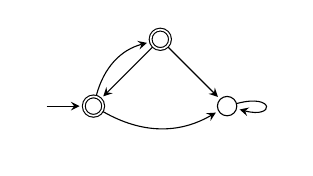
\begin{tikzpicture}[>=stealth, shorten >=1pt, auto, node distance=1.2cm,initial text={}]
\node[state, initial, accepting, inner sep=1pt, minimum size=7pt] (S0) {};
\node[state, accepting, inner sep=1pt, minimum size=7pt][above right of=S0] (S1) {};
\node[state, inner sep=1pt, minimum size=7pt][below right of=S1] (S2) {};
\path[->] (S0) edge [bend left] node {} (S1)
               edge [bend right] node [swap] {} (S2)
		  (S1) edge node [pos=.2]{} (S0)
		       edge node {} (S2)
		  (S2) edge [loop right] node {} ();
\end{tikzpicture} \end{center}
\caption{Automata for the languages , , and , .}

\label{fig:prefe2} 
\end{figure}



\begin{corollary}
\label{cor:dprefinite}
  If  is a finite language, then .
\end{corollary}

The state complexity of the  operation is given by the following theorem.
\begin{theorem}
\label{theo:scdpre}
If  is recognized by a minimal \dfa with  states, then
 .
\end{theorem}
\begin{proof}
 If both  and  do not have  as a quotient, then  
and only one state is needed for a \dfa accepting . 
Otherwise, let  be the minimal \dfa recognizing  with .
We have that at least one of  or  has a dead state. 
To obtain a \dfa for  one needs only to  consider all states of  final, except the dead state, if it exists. 
To get a \dfa for , we also need to exclude from the set of final states the possible dead state of the \dfa , recognizing , which coincides with , except that the set of final states is . Tightness is achieved  for the family of languages , which are prefix closed,~\cite{brzozowski14:_quotien_compl_of_closed_languag}.\end{proof}

In Section~\ref{sec:minDist}, we considered the language of the shortest words that distinguish pairs of left quotients of , . 
In this case, we can define , where
 if , and minimum is considered with respect to the quasi-lexicographical order. 
Using Equation (\ref{eq:dpredis}), one can have a finite set of words that distinguish between right quotients, namely .
However, using the notion of atoms we can compute directly .
As we seen before,  distinguishes between pairs of atoms of . To estimate the number of elements of , we recall the relation between atoms and right quotients.

 Let  be the minimal \dfa recognizing  and let ,  be the left quotients of . 
Each atom can be characterized by a set  such that 
.
Every   belongs exactly to one atom , and if , i.e, , 
then  and  belong to the same atom. 
Thus, the minimal word that distinguishes two distinct right quotients with correspondent  sets  and  is 
 
where  for  and . 
Therefore . 
Using Theorem~\ref{theo:mindist_upp_bound_set}, it follows that . 
We also have that  is prefix closed, ,  
and we can reach the fixed point in maximum  iterations, using Theorem~\ref{theo:fpdismin} and 
Theorem~\ref{theo:fpdismint}, with  .

\subsection{Two-sided Distinguishability}
\label{sec:twosideddis}
Given a language , we can define the (Myhill-Nerode) equivalence relation on , 
 if and only if 
. If  is regular,  is of finite index and for , the two-sided quotient  corresponds to an equivalence class of .
We note that .
Two-sided quotients were recently used to define biautomata, which deterministic versions recognize exactly regular languages,~\cite{holzer13:_nondet_biaut_and_their_descr_compl,klima12:_biaut}, and \emph{couple} \nfas,
  which can recognize linear languages,~\cite{champarnaud13:_two_sided_deriv_for_regul}.

We define
the \emph{two-sided distinguishability language} of  by 

\noindent It is immediate that 

and


Please note that  for all regular languages ,  and  . 
If  has  as a (left) quotient, then  is also a two-sided quotient. 
The following lemmata show that  is always an  operation.

\begin{lemma}
\label{lem:qinf}
Let  be a regular language. If  does not have  as a quotient, .
\end{lemma}
\begin{proof} 
Since  is not a quotient of , it follows that  , therefore .
\end{proof}

\begin{lemma}
\label{lem:qeinf}
Let  be a regular language. If  has  as a  quotient, then  .
\end{lemma}
\begin{proof}
We know that , thus .
\end{proof}


If  is infix closed, then  is also suffix and prefix closed. 
Excluding , the fixed points of  are exactly the infix-closed languages. 
To see that, by the previous lemma we have:


\begin{lemma}
\label{lem:inffixpoint}
If  is a infix-closed regular language and   has a  as a quotient, then .
\end{lemma}

\begin{lemma}
\label{lem:dinfpe}
Let  be a regular language. If  , then 
 has  as a quotient.
 \end{lemma}
\begin{proof}
Assume  does not have  as a quotient.
By Lemma~\ref{lem:qinf}, it follows  , thus  would not be a fixed point of .
\end{proof}



From these two lemmata, one has
\begin{theorem}
\label{theo:dinffixpoint}
If  is a regular language different from ,  if and only if  is infix closed.
\end{theorem}

\begin{corollary}
\label{cor:dinffinite}
  If  is a finite language, then .
\end{corollary}

In case , . Because,
, we have .
This result can be generalized for all regular languages , such that .

\begin{corollary}
\label{cor:f2f}
Given  a regular language , if , then . 
\end{corollary}
\begin{proof}
If , then either  or  has  as a quotient.
Hence,    and  or
  and  .
\end{proof}



The state complexity of  coincides with the state complexity of the  operation.

\begin{theorem}
\label{theo:scdinf}
If  is recognized by a minimal \dfa with  states, then
.
\end{theorem}

\begin{proof}
 If both  and  do not have  as a quotient, then , 
therefore only one state is needed for a \dfa accepting . 
Otherwise, let  be the minimal \dfa recognizing  with , 
hence at least one of  or  has a dead state.
An \nfa recognizing  can be obtained by marking as initial and final all states of  and deleting the possible dead states.
The correspondent \dfa has at most  states,~\cite{brzozowski14:_quotien_compl_of_closed_languag}. 
An analogous construction can be used for . 
Considering Lemma~\ref{lem:qinf} and Lemma~\ref{lem:qeinf}, a \dfa for  is one of the above. 
Tightness is achieved for the family of languages recognized by \dfas represented in Figure~\ref{fig:upsuffe}.
\end{proof}

In this case, we can also define
,
where 
. Although it is easy to see that  enjoy similar properties of  and , we leave open how to compute this set.



\section{Conclusion}
\label{sconc}


In this paper we have introduced two new operations on regular languages
that help us distinguish non-equivalent words under Myhill-Nerode equivalence.
The first one  finds all these words and the second one 
produces only the minimal ones, where minimum is considered with respect 
to the quasi-lexicographical order.
Both have fixed points under iteration. 
The number of iterations  until a fixed point is reached is bounded by  for
the case of , and it is bounded by the state complexity 
of the starting language for .
A full characterization of the fixed points of  is provided. 
Brzozowski's universal witness  reaches the upper-bound of ,
for the state complexity of .
In the case of  operation, the maximum number of words in 
the language is , where  is the state complexity of the original language.
We used  to recover the original language  as an -cover language of 
an initial segment of the language, where words have length at most , by generating 
words in the language up to length , where  is the length of the 
longest word in .
We have generalized some results for these type of operations with arbitrary closures and 
Boolean operations.
We have extended the study to infix and prefix operators to distinguish right quotients and 
atoms of a language.

As open problems and future work we can consider the state complexity of combined
operations, when one of them is in the set .
It worth mentioning that recovering the whole language from a finite number of words in the language
 is very useful in learning algorithms, thus  it would be useful to study all 
conditions that can help us to reconstruct it if we know some of the distinguishability languages.
Finite languages have the particularity that distinguishability operation reduces to the suffix one.
What would be corresponding operation for cover automata for finite languages and dissimilarity operation? 


\newcommand{\etalchar}[1]{}
\begin{thebibliography}{BBMR14}

\bibitem[BBH{\etalchar{+}}85]{blumer85:_small_autom_recog_subwor_of_text}
Anselm Blumer, J.~Blumer, David Haussler, Andrzej Ehrenfeucht, M.~T. Chen, and
  Joel~I. Seiferas.
\newblock The smallest automaton recognizing the subwords of a text.
\newblock {\em Theor. Comput. Sci.}, 40:31--55, 1985.

\bibitem[BBMR14]{bell14:_symmet_group_and_quotien_compl}
Jason Bell, Janusz~A. Brzozowski, Nelma Moreira, and Rog{\'e}rio Reis.
\newblock Symmetric groups and quotient complexity of boolean operations.
\newblock In Javier Esparza, Pierre Fraigniaud, Thore Husfeldt, and Elias
  Koutsoupias, editors, {\em Proc. 41st ICALP}, volume 8573 of {\em LNCS},
  pages 1--12. Springer, 2014.

\bibitem[BGS11]{brzozowski11:_closur_in_formal_languag_and_kurat_theor}
Janusz~A. Brzozowski, Elyot Grant, and Jeffrey Shallit.
\newblock Closures in formal languages and {Kuratowski}'s theorem.
\newblock {\em Int. J. Found. Comput. Sci.}, 22(2):301--321, 2011.

\bibitem[BJZ14]{brzozowski14:_quotien_compl_of_closed_languag}
Janusz~A. Brzozowski, Galina Jir{\'a}skov{\'a}, and Chenglong Zou.
\newblock Quotient complexity of closed languages.
\newblock {\em Theory Comput. Syst.}, 54(2):277--292, 2014.

\bibitem[Brz13]{brzozowski13:_in_searc_of_most_compl_regul_languag}
Janusz~A. Brzozowski.
\newblock In search of most complex regular languages.
\newblock {\em Int. J. Found. Comput. Sci.}, 24(6):691--708, 2013.

\bibitem[BT11]{brzozowski11:_theor_of_atomat}
Janusz~A. Brzozowski and Hellis Tamm.
\newblock Theory of {\'a}tomata.
\newblock In Giancarlo Mauri and Alberto Leporati, editors, {\em Proc. 15th
  DLT}, volume 6795 of {\em LNCS}, pages 105--116. Springer, 2011.

\bibitem[BT13]{brzozowski13:_compl_of_atoms_of_regul_languag}
Janusz~A. Brzozowski and Hellis Tamm.
\newblock Complexity of atoms of regular languages.
\newblock {\em Int. J. Found. Comput. Sci.}, 24(7):1009--1028, 2013.

\bibitem[C{\^a}m13]{campeanu13:_cover_languag_and_implem}
Cezar C{\^a}mpeanu.
\newblock Cover languages and implementations.
\newblock In Stavros Konstantinidis, editor, {\em Proc. 18th CIAA}, volume 7982
  of {\em LNCS}, page~1. Springer, 2013.

\bibitem[CDJM13]{champarnaud13:_two_sided_deriv_for_regul}
Jean{-}Marc Champarnaud, Jean{-}Philippe Dubernard, Hadrien Jeanne, and Ludovic
  Mignot.
\newblock Two-sided derivatives for regular expressions and for hairpin
  expressions.
\newblock In Adrian~Horia Dediu, Carlos Mart{\'{\i}}n{-}Vide, and Bianca
  Truthe, editors, {\em Proc. 7th {LATA} 2013}, volume 7810 of {\em Lecture
  Notes in Computer Science}, pages 202--213. Springer, 2013.

\bibitem[CP03]{CezarAndreiCount}
Cezar C\^ampeanu and Andrei P\u{a}un.
\newblock Counting the number of minimal {DFCA} obtained by merging states.
\newblock {\em Int. J. Found. Comput. Sci.}, 14(6):995--1006, 2003.

\bibitem[DESW11]{demaine11:_remar_separ_words}
Erik~D. Demaine, Sarah Eisenstat, Jeffrey Shallit, and David~A. Wilson.
\newblock Remarks on separating words.
\newblock In Markus Holzer, Martin Kutrib, and Giovanni Pighizzini, editors,
  {\em Proc. 13th DCFS}, volume 6808 of {\em LNCS}, pages 147--157. Springer,
  2011.

\bibitem[Gin58]{ginsburg58:_lengt_of_small_unifor_exper}
Seymour Ginsburg.
\newblock On the length of the smallest uniform experiment which distinguishes
  the terminal states of a machine.
\newblock {\em J. ACM}, 5(3):266--280, 1958.

\bibitem[GS61]{Ginsburg1960:InputSemigroup}
Seymour Ginsburg and EH~Spanier.
\newblock Distinguishability of a semi-group by a machine.
\newblock {\em Proceedings of the American Mathematical Society},
  12(4):661--668, 1961.

\bibitem[HJ13]{holzer13:_nondet_biaut_and_their_descr_compl}
Markus Holzer and Sebastian Jakobi.
\newblock Nondeterministic biautomata and their descriptional complexity.
\newblock In Helmut J{\"{u}}rgensen and Rog{\'{e}}rio Reis, editors, {\em Proc.
  15th {DCFS} 2013}, volume 8031 of {\em Lecture Notes in Computer Science},
  pages 112--123. Springer, 2013.

\bibitem[KP12]{klima12:_biaut}
Ondrej Kl{\'{\i}}ma and Libor Pol{\'{a}}k.
\newblock On biautomata.
\newblock {\em {RAIRO} - Theor. Inf. and Applic.}, 46(4):573--592, 2012.

\bibitem[Kur22]{Kuratowski1922}
C.~Kuratowski.
\newblock Sur l’operation  de l’analysis situs.
\newblock {\em Fund. Math.}, 3:182--199, 1922.

\bibitem[MMW09]{mohri09:_gener_suffix_autom_const_algor}
Mehryar Mohri, Pedro Moreno, and Eugene Weinstein.
\newblock General suffix automaton construction algorithm and space bounds.
\newblock {\em Theor. Comput. Sci.}, 410(37):3553--3562, 2009.

\bibitem[RV12]{restivo12:_graph_theor_approac_to_autom_minim}
Antonio Restivo and Roberto Vaglica.
\newblock A graph theoretic approach to automata minimality.
\newblock {\em Theor. Comput. Sci.}, 429:282--291, 2012.

\bibitem[Sak09]{sakarovitch09:_elemen_of_autom_theor}
Jacques Sakarovitch.
\newblock {\em Elements of Automata Theory}.
\newblock Cambridge University Press, 2009.

\bibitem[Sem06]{JoseSempere}
Jos{\'e}~M. Sempere.
\newblock Learning reversible languages with terminal distinguishability.
\newblock volume 4201 of {\em LNCS}, pages 354--355. Springer, 2006.

\bibitem[Yu97]{yu97:_handb_formal_languag}
S.~Yu.
\newblock Regular languages.
\newblock In Grzegorz Rozenberg and Arto Salomaa, editors, {\em Handbook of
  {F}ormal {L}anguages}, volume~1, pages 41--110. Springer, 1997.

\end{thebibliography}
\end{document}
